\documentclass[11pt,a4paper]{article}

\usepackage[spanish,es-nodecimaldot]{babel}
\usepackage[utf8]{inputenc}
\usepackage[T1]{fontenc}
\usepackage{lmodern}
\usepackage[a4paper,margin=2.3cm]{geometry}
\usepackage{amsmath,amssymb,mathtools}
\usepackage{booktabs}
\usepackage{array}
\usepackage{enumitem}
\usepackage{microtype}
\usepackage[hidelinks]{hyperref}
\usepackage{float}
\usepackage{xcolor}

\setlength{\parindent}{1em}
\setlength{\parskip}{0.25em}
\setlist[itemize]{noitemsep,topsep=2pt}
\setlist[enumerate]{noitemsep,topsep=2pt}

\title{Resolución de una instancia del Problema del Agente Viajero (TSP) con la heurística de Aceptación por Umbrales}
\author{Alvarez Caamaño Luis Enrique}
\date{}

\begin{document}
\maketitle

\begin{abstract}
En este trabajo se presenta la implementación de una heurística de
Aceptación por Umbrales para resolver una variante del Problema del
Agente Viajero (TSP). El problema consiste en encontrar una
trayectoria de longitud mínima que visite exactamente una vez un
conjunto seleccionado de ciudades de una base de datos, sin requerir
el regreso a la ciudad inicial. Las ciudades y sus conexiones se
obtienen de una base de datos, mientras que las distancias geográficas
entre ciudades no conectadas se emplean para construir una función de
costo aumentada que penaliza soluciones no factibles. La solución se
representa como una permutación de id's de ciudades y su vecindario se
genera mediante el intercambio aleatorio de dos posiciones.
\end{abstract}

\section{Introducción}





Muchos problemas de optimización combinatoria pueden formularse como
la búsqueda de una solución de costo mínimo entre un conjunto de
soluciones cuya enumeración exhaustiva resulta impráctica. En este
contexto es importante distinguir entre los problemas de la clase NP y
los problemas NP-duros.


La clase NP son problemas de decisión para los cuales una máquina de
Turing no determinista puede resolverlos en tiempo polinomial o,
equivalentemente, que dada una solución o certificado para una
instancia de un problema, se puede verificar su validez en tiempo
polinomial mediante una máquina de Turing determinista. Sin embargo,
esta afirmación no dice nada sobre cómo encontrar dicha solución o
sobre si es posible encontrarla en tiempo polinomial.

Por otro lado, un problema está en NP-completo si dicho problema
pertenece a NP y, además, cualquier problema de NP puede reducirse a
él mediante una reducción en tiempo polinomial. Además, un problema es
NP-duro si al menos es tan difícil como cualquier problema de NP, es
decir, si cualquier problema de NP puede reducirse a él en tiempo
polinomial. A diferencia de los problemas NP-completos, un problema
NP-duro no tiene por qué ser un problema de decisión, sino que también
puede ser un problema de optimización, entre otros.

Dado que computacionalmente puede resultar impráctico utilizar
algoritmos deterministas para resolver instancias de problemas
NP-duros, en la práctica se suele recurrir a métodos como heurísticas,
metaheurísticas o algoritmos de aproximación para obtener soluciones
de buena calidad en un tiempo razonable.


El Problema del Agente Viajero (TSP) busca determinar la ruta de costo
minimo que visite un conjunto de ciudad. El problema clásico es
encontrar un ciclo Hamiltoniano que empiece en una ciudad y regrese a
dicha ciudad. Sin embargo para este proyecto se buscarán soluciones
para una variante de TSP, es decir, en vez de un ciclo se quiere
encontrar una trayectoría de distancia mínima. \cite{materialTsp}.


La instancia se representa mediante una gráfica ponderada que contiene
las ciudades y sus conexiones. La gráfica original no necesariamente
es completa. Para poder evaluar cualquier permutación de ciudades, se
utiliza una gráfica completa auxiliar y una función de peso
aumentada. Si dos ciudades están conectadas en la gráfica original, se
conserva su distancia; si no existe la conexión, se utiliza la
distancia natural multiplicada por una distancia máxima de la
instancia. De esta forma, las soluciones que emplean conexiones
inexistentes reciben un costo mayor y son penalizadas durante la
búsqueda \cite{materialTsp}.

Debido a la naturaleza combinatoria del problema, el número de
permutaciones posibles crece factorialmente con el número de
ciudades. Por ello, en lugar de explorar exhaustivamente el espacio de
soluciones, se utiliza una heurística de Aceptación por Umbrales,
presentada en el material como una variante del Recocido Simulado más
sencilla de implementar \cite{materialThreshold}.
La idea central es aceptar tanto soluciones que sean mejores que la solución
actual, pero también aceptar permutaciones que sean ligeramente peores bajo
cierto umbral. Sin embargo cuando más iteraciones se haga más restrictivo se
vuelve el algoritmo y dicho umbral disminuye.

\section{Modelo del problema y función de costo}

Sea $S$ el conjunto de ciudades seleccionadas y $G=(S,E)$ la gráfica
ponderada de las conexiones disponibles. Una solución es una
permutación
\[
P=(v_{\rho(1)},v_{\rho(2)},\ldots,v_{\rho(k)}).
\]
La solución es factible si cada par consecutivo de ciudades está
conectado en $G$, es decir,
\[
(v_{\rho(i-1)},v_{\rho(i)})\in E,\qquad i=2,\ldots,k.
\]

Para permitir la evaluación de soluciones no factibles, se define una
función de peso aumentada $w_S$ sobre la gráfica completa:
\[
w_S(u,v)=
\begin{cases}
 w(u,v), & \text{si }(u,v)\in E,\\[4pt] d(u,v)\,\max d(S), & \text{en
   otro caso},
\end{cases}
\]
donde $d(u,v)$ representa la distancia natural calculada a partir de
las coordenadas geográficas de las ciudades. La distancia máxima se
toma únicamente entre pares conectados de la instancia
\cite{materialTsp}.

Además, se define el normalizador $N(S)$ como la suma de las $k-1$
aristas más pesadas existentes entre las ciudades de la instancia (o
de todas ellas si hay menos de $k-1$). La función objetivo utilizada
por el programa es entonces
\[
f(P)=\frac{1}{N(S)}\sum_{i=2}^{k}
w_S\bigl(v_{\rho(i-1)},v_{\rho(i)}\bigr).
\]
Esta normalización permite interpretar las soluciones factibles en una
escala comparable entre instancias. Las factibles quedan acotadas por
$1$ y las no factibles reciben un valor superior a $1$
\cite{materialTsp}.

\section{Heurística de Aceptación por Umbrales}

La heurística parte de una solución inicial $s$ y de un umbral inicial $T$. En cada paso se genera aleatoriamente una solución vecina $s'$ y se acepta cuando
\[
f(s')\leq f(s)+T.
\]
Por lo tanto, una solución peor puede ser aceptada si la diferencia de costo es suficientemente pequeña. Esta característica permite escapar de mínimos locales durante las primeras etapas de la búsqueda. El umbral se reduce gradualmente mediante un factor $\phi$, de modo que
\[
T_{j+1}=\phi T_j,\qquad 0<\phi<1.
\]
La ejecución termina cuando $T \varepsilon$, además de las condiciones de paro establecidas para completar un lote \cite{materialThreshold}.


\section{Diseño e implementación}



\subsection{Arquitectura e implementación}

El programa se organizó en módulos con responsabilidades separadas. El
módulo domain contiene los elementos propios del problema:
ciudades, conexiones, rutas, la gráfica y la instancia del TSP. El
módulo database se encarga exclusivamente de obtener la
información de las ciudades y sus conexiones desde la base de datos
SQLite. Por otro lado, input procesa la instancia del
problema y los parámetros de configuración proporcionados por el
usuario. Finalmente, solver contiene la implementación de la
heurística de Aceptación por Umbrales.

La construcción de una instancia sigue el siguiente flujo:

\begin{center}
\texttt{archivo .tsp} $\rightarrow$ \texttt{parser} $\rightarrow$
\texttt{lista de ciudades} $\rightarrow$ \texttt{database}
$\rightarrow$ \texttt{ciudades y conexiones} $\rightarrow$
\texttt{Problem} $\rightarrow$ \texttt{ThresholdAccepting}
\end{center}

La ejecución comienza en main, que coordina estos
componentes, construye la instancia del problema y crea una solución
inicial. Posteriormente, la instancia se entrega al solver
junto con los parámetros y la semilla aleatoria, y este ejecuta la
búsqueda hasta finalizar el criterio de terminación, conservando la
mejor solución encontrada durante el proceso.

Los parámetros del algoritmo pueden establecerse mediante un archivo
de configuración; cuando éste no se proporciona, el programa utiliza
valores definidos por defecto. Cabe aclarar que la representación de
la gráfica está limitada a lo más a 150 vértices y se utiliza una
matriz de adyacencia. Se optó por este diseño debido a que el número
de vértices es relativamente pequeño y una matriz permite acceder
directamente a la conexión entre dos vértices en tiempo
constante. Además, al estar sus elementos almacenados de forma
contigua en memoria, se puede aprovechar una mejor localidad de caché
que en estructuras basadas en nodos enlazados, donde los elementos
pueden encontrarse en diferentes posiciones de memoria.



\section{Resultados}

La evaluación experimental debe considerar tanto la calidad de las
soluciones como el comportamiento de la búsqueda. Debido al carácter
estocástico de la heurística, una ejecución aislada no basta para
describir completamente el comportamiento del método; por ello,
conviene repetir la ejecución con distintas semillas y conservar los
parámetros utilizados en cada corrida.

Las métricas principales a reportar saon la evaluación final $f(P)$,
la factibilidad de la solución, el número de lotes procesados y,
cuando sea posible, el tiempo de ejecución. También resulta útil
registrar la evolución del mejor costo encontrado y del umbral $T$
durante la ejecución.


\subsection{Interpretación de los resultados}

En una de las ejecuciones realizadas, utilizando la semilla
\(1432277707348111984\), la heurística de Aceptación por Umbrales
encontró una solución con un costo de

$$ f(P)=98\,973\,851.12$$

y una evaluación normalizada de

$$ \operatorname{Evaluación}(P)=0.1369693 $$

La evaluación se obtiene mediante la expresión

$$ \operatorname{Evaluación}(P)=\frac{f(P)}{N(S)} $$

donde \(N(S)\) es el normalizador de la instancia. Debido a que el
valor obtenido es menor que \(1\), el resultado es consistente con una
solución factible.

La solución obtenida fue marcada como factible, lo que significa que
para cada par de ciudades consecutivas en la trayectoria existe una
conexión en el grafo original. La ruta contiene las 150 ciudades de la
instancia, visitando cada una exactamente una vez. Además, la
trayectoria no regresa a la ciudad inicial, ya que el problema
considerado corresponde a la búsqueda de un camino Hamiltoniano mínimo
y no de un ciclo Hamiltoniano.

Es importante señalar que el valor \(98\,973\,851.12\) corresponde a
la mejor solución encontrada durante esta ejecución y no implica que
se haya obtenido necesariamente la solución óptima global. La semilla
utilizada se conserva para permitir la reproducción de la misma
corrida.

En una corrida se consiguió la siguiente evaluación: $0.13676796147292805$, con el siguiente camino:

\begin{center}
\small
\texttt{494, 495, 167, 328, 326, 1037, 169, 1073, 330, 819, 655, 818, 666,}\
\texttt{658, 166, 822, 74, 1001, 297, 980, 336, 840, 350, 670, 327, 511,}\
\texttt{504, 500, 825, 20, 660, 510, 343, 985, 674, 334, 999, 8, 662,}\
\texttt{331, 995, 837, 979, 493, 509, 329, 163, 172, 182, 496, 839,}\
\texttt{19, 505, 168, 508, 986, 1, 829, 657, 663, 661, 832, 9, 815,}\
\texttt{184, 667, 656, 2, 173, 673, 507, 7, 823, 678, 816, 187, 982,}\
\texttt{14, 181, 332, 345, 820, 26, 654, 490, 653, 344, 665, 676, 22,}\
\texttt{185, 991, 351, 1004, 6, 5, 978, 352, 668, 176, 23, 988, 981,}\
\texttt{990, 353, 27, 333, 3, 165, 174, 4, 489, 817, 347, 499, 492,}\
\texttt{25, 491, 984, 349, 1003, 11, 164, 501, 17, 444, 826, 244, 339,}\
\texttt{1038, 12, 828, 502, 340, 675, 186, 520, 16, 671, 179, 652,}\
\texttt{1075, 483, 512, 821, 75, 346, 183, 77, 171.}
\end{center}

La semilla utilizada para esta corrida no pudo ser recuperada, por lo que no fue posible reproducir exactamente este resultado. Sin embargo, se conserva la evaluación obtenida y el camino encontrado por el algoritmo.

La representación gráfica del camino obtenido se muestra:

\begin{figure}[ht]
\centering
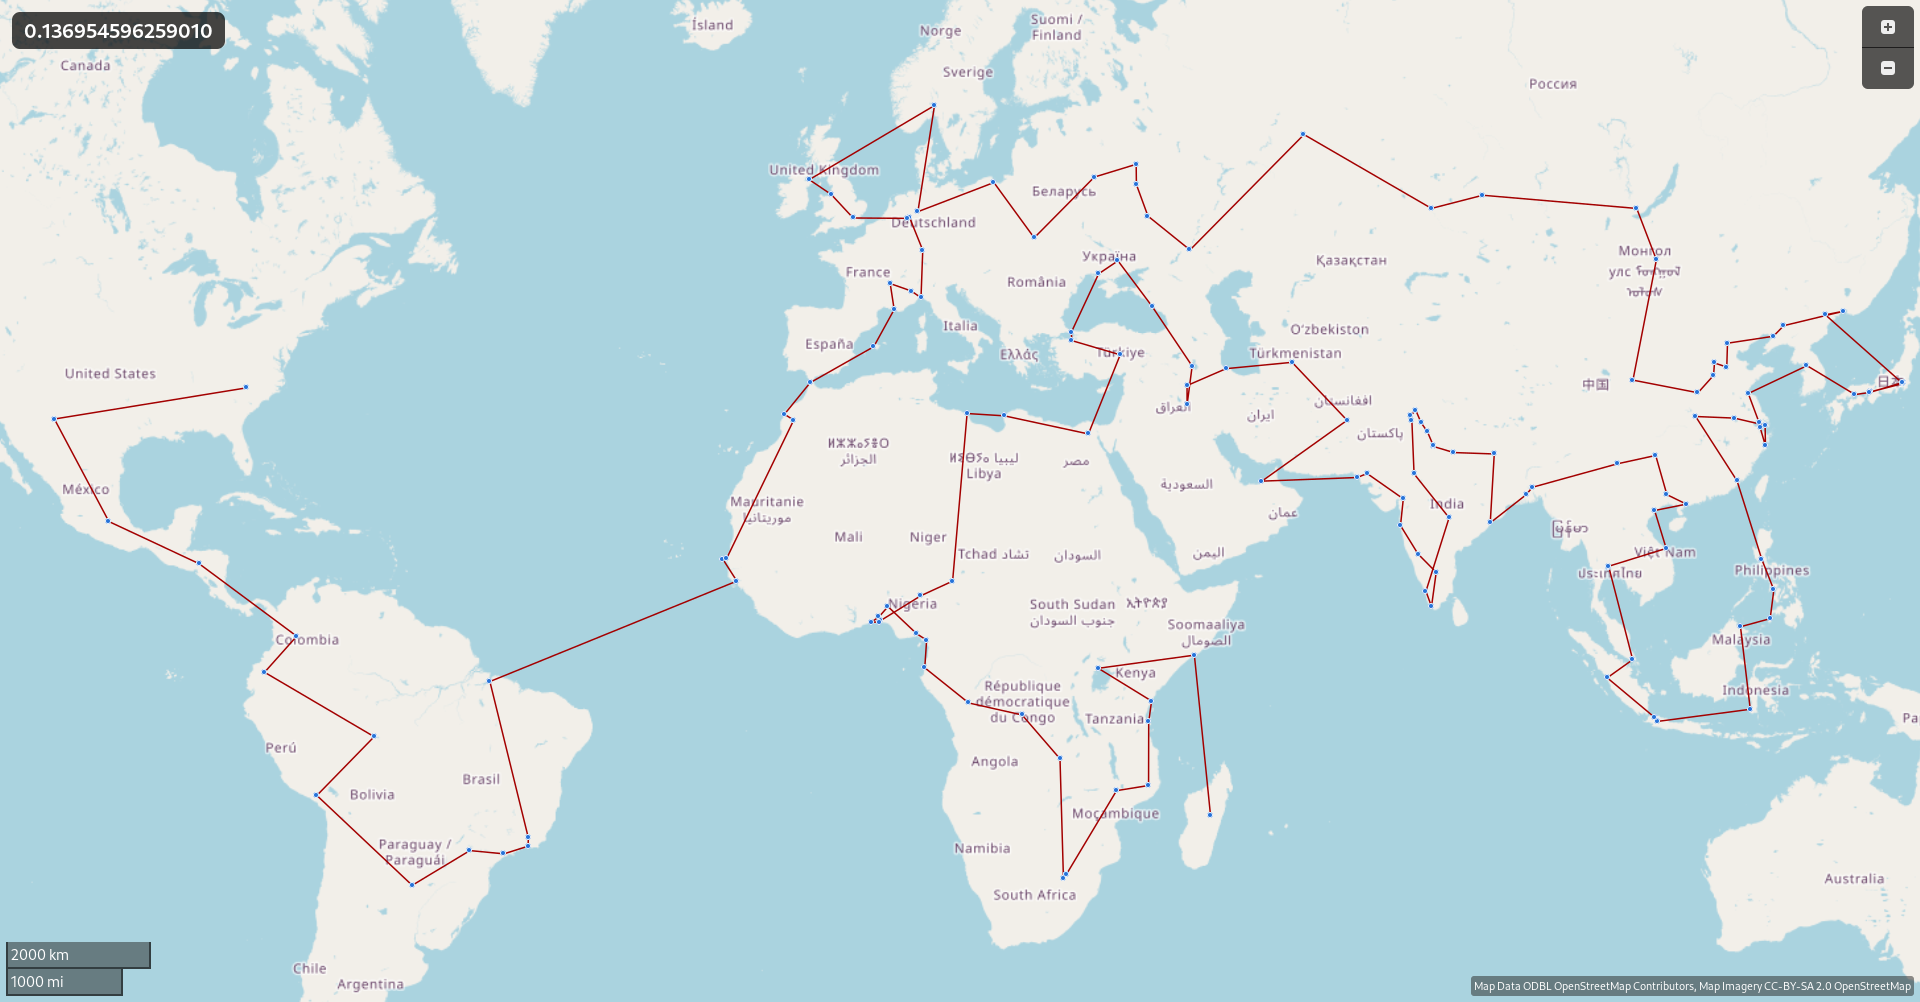
\includegraphics[width=0.5\textwidth]{ruta_tsp.png}
\caption{Mapa correspondiente al camino obtenido por la heurística de Aceptación por Umbrales.}
\label{fig:mapa-ruta}
\end{figure}






\section{Conclusiones}

La implementación desarrollada permite aplicar una heurística de
Aceptación por Umbrales a una variante del Problema del Agente Viajero
en la que no se requiere regresar al punto de partida. La función de
costo utilizada incorpora información de las conexiones reales entre
ciudades y una penalización basada en la distancia geográfica para las
conexiones inexistentes,  de manera que el algoritmo puede explorar el
espacio completo de permutaciones sin perder el objetivo de encontrar
soluciones factibles.

El enfoque heurístico permite trabajar con instancias para las cuales
una enumeración exhaustiva de todas las permutaciones no resulta
práctica. Al mismo tiempo,  el comportamiento del método depende de sus
parámetros y de la secuencia pseudoaleatoria,  por lo que la calidad de
una solución debe interpretarse junto con las condiciones concretas de
la ejecución. El uso de semillas explícitas facilita reproducir los
experimentos y comparar cambios en la configuración.



\begin{thebibliography}{9}

\bibitem{materialTsp}
Material del curso, 
\textit{El Problema del Agente Viajero},  Capítulo 4, 
secciones sobre soluciones,  función de costo y vecinos.

\bibitem{materialThreshold}
Material del curso, 
\textit{Aceptación por Umbrales},  Capítulo 7, 
secciones sobre la heurística,  lotes,  temperatura inicial y parámetros.

\bibitem{gareyjohnson}
M. R. Garey and D. S. Johnson, 
\textit{Computers and Intractability: A Guide to the Theory of NP-Completeness}, 
W. H. Freeman, 1979.

\end{thebibliography}

\end{document}
